\documentclass[12pt]{article}
\usepackage[utf8]{inputenc}
\usepackage[T1]{fontenc}
\usepackage{amsmath}
\usepackage{physics}

\usepackage{amsfonts}
\usepackage{amssymb}
\usepackage[version=4]{mhchem}
\usepackage{stmaryrd}
\usepackage{hyperref}
\hypersetup{colorlinks=true, linkcolor=blue, filecolor=magenta, urlcolor=cyan,}
\urlstyle{same}
\usepackage{graphicx}
\usepackage[export]{adjustbox}

\usepackage{listings} % Required for insertion of code
\usepackage{xcolor} % Required for custom colors

% Define custom colors
\definecolor{codegreen}{rgb}{0,0.6,0}
\definecolor{codegray}{rgb}{0.5,0.5,0.5}
\definecolor{codepurple}{rgb}{0.58,0,0.82}
\definecolor{backcolour}{rgb}{0.95,0.95,0.92}

% Setup the style for code listings
\lstdefinestyle{mystyle}{
    backgroundcolor=\color{backcolour},   
    commentstyle=\color{codegreen},
    keywordstyle=\color{magenta},
    numberstyle=\tiny\color{codegray},
    stringstyle=\color{codepurple},
    basicstyle=\ttfamily\footnotesize,
    breakatwhitespace=false,         
    breaklines=true,                 
    captionpos=b,                    
    keepspaces=true,                 
    numbers=left,                    
    numbersep=5pt,                  
    showspaces=false,                
    showstringspaces=false,
    showtabs=false,                  
    tabsize=2
}

% Activate the style
\lstset{style=mystyle}

\graphicspath{ {./images/} }

\title{Ch/ChE 164 Winter 2022 Final Project \\
 The Statistical Thermodynamics of $\mathrm{He}^{3}-\mathrm{He}^{4}$ Mixtures }

\author{}
\date{}


\begin{document}
\maketitle
Due Date: Friday March 15, 2024 @ 11:59pm PT

An interesting and instructive problem in statistical mechanics is the fluid-superfluid transition of $\mathrm{He}^{4}$ at low temperatures. This transition is typically continuous (2nd-order), but becomes discontinuous (1st-order) in the presence of a critical amount of $\mathrm{He}^{3}$ impurities. In this project, we aim to model and understand this behavior by both deriving analytical results, and implementing simulation methods.

\begin{itemize}
  \item For a really cool visual of the transition, watch the video at this link: \href{https://youtu.be/}{https://youtu.be/} 2Z6UJbwxBZI.
\end{itemize}

The system to model is described as follows:

\begin{itemize}
  \item The system can be described as a lattice gas. From class, we know that the lattice-gas model is isomorphic with the Ising model. In this problem, we can treat the helium fluid/superfluid using a variation of the spin- 1 Ising model. We say $\mathrm{He}^{4}$ particles can have spin $s= \pm 1$, whereas $\mathrm{He}^{3}$ particles have spin $s=0$. We thus interpret the problem as a "diluted" Ising model where the presence of the impurities $(s=0)$ serve only to disrupt the interactions. The fluid/superfluid transition then becomes the disorder/order transition.
  \item The lattice has coordination number $z$.
  \item For convenience, we label $\mathrm{He}^{4}$ as Type $\mathbf{A}$ and $\mathrm{He}^{3}$ as Type B.
  \item The Type A spins interact with each other through magnetic nearest-neighbor interactions with strength $J \geq 0$ (ferromagnetic), whereas Type B spins have no magnetic interactions and are taken simply as non-interactive impurities.
  \item The spins are not subjected to an external magnetic field, i.e. $h=0$.
  \item We can consider the system in the constrained grand canonical ensemble, where $N_{A}+N_{B}=N$ with $N$ fixed. In the lattice model, $N$ replaces $V$ since $N=V / v_{0}$ where $v_{0}$ is the size of a lattice site.
\end{itemize}

\section{}
\begin{enumerate}
  \item Deriving the free energy of the diluted Ising model.
\end{enumerate}
\subsection{}
a) Determine the characteristic variables of the system in the grand canonical ensemble.\\
As always, we will have the temperature as one of these. In this case, we are told that the total number of particles will replace the volume, so the second variable is $N$. Finally, we are interested in the chemical potentials of both particles, so we will have $\mu_{A}$ and $\mu_{B}$ as the third and fourth variables.
\subsection{}
b) Write the Hamiltonian in terms of the spin-state of the system. Remember, only neighbors that are both Type A interact.\\
There is no external magnetic field for this system, so the Hamiltonian only has the interaction term. The Hamiltonian is given by:
\begin{equation}
  \mathcal{H}=-K\sum_{i = 0}^{N_{A}} \sum_{j=0}^{z-1} \sum_{s_i = \pm 1} \sum_{s_j = \pm 1}   \delta _{s_{i},s_{j}} \tag{1}
\end{equation}
where $K$ is the interaction strength, $N_{A}$ is the number of Type A particles, $z$ is the coordination number, and $s_{i}$ and $s_{j}$ are the spins of the particles. The reasoning is as follows: for the first summation we want to go through all the particles of type A, and for each of them we want to go through all the neighbors, as represented by the second summation. Finally, we want to check whether the spins are the same and if they are, then the interaction provides a contribution to the Hamiltonian.
\subsection{}
c) Define the relative magnetization $m$, and the Type A number fraction $x$ :


\begin{align*}
m & =\frac{\mathcal{M}}{N_{A}}=\frac{\sum_{i=1}^{N} s_{i}}{N_{A}}=\frac{\sum_{i=1}^{N} s_{i}}{x N} ; \quad-1 \leq m \leq 1  \tag{1}\\
x & =\frac{N_{A}}{N} ; \quad 0 \leq x \leq 1 \tag{2}
\end{align*}


Using the mean field approximation, write an expression for the average Hamiltonian in terms of $m$ and $x$. In other words, eliminate all summations over the spin-state.\\
In a man field approximation, the average field filled by a single particle is:
\begin{equation}
  h_i^{\prime} = K \sum_{j=0}^{z-1} \delta _{s_{i},s_{j}} \tag{3}
\end{equation}
\subsection{}
d) Write an expression of the Gibbs entropy in terms of $m$ and $x$.\\
The Gibbs entropy is given by:
\begin{equation}
  S=-k \sum_{i} \left[p_{i} \ln p_{i}+\left(1-p_{i}\right) \ln \left(1-p_{i}\right)\right] \tag{4}
\end{equation}
where $p_{i}$ is the probability of the system being in the $i$-th state.
\subsection{}
e) Write the variational free energy, $G$. In addition to the variables characteristic to the ensemble, the free energy should also depend on $m$ and $x$.\\
The free energy is given by:
\begin{equation}
  G=E-TS
\end{equation}
where $E$ is the average Hamiltonian and $S$ is the Gibbs entropy. We need to find the average energy and the entropy of the previous problem.
\subsection{}

f) Express the free energy as a dimensionless free energy per particle, $g$. Define new scaled parameters.


\begin{equation*}
g \equiv \frac{G}{N k T}, \quad \alpha \equiv \frac{z J}{k T}, \quad \mu \equiv \frac{\Delta \mu}{k T} \equiv \frac{\mu_{A}-\mu_{B}}{k T} \tag{3}
\end{equation*}
Now, we want to manipulate the expression for the free energy that we just got.

\begin{enumerate}
  \setcounter{enumi}{1}
  \item Analyzing the free energy
\end{enumerate}

a) State the conditions for phase equilibrium.

b) Minimize the free energy with respect to $m$ to obtain an implicit relationship between $m$ and $x$, i.e. $F(m, x)=0$.

c) Minimize the free energy with respect to $x$ to obtain an equation for $\mu=\mu(m, x)$.

d) With these equations in hand, plot the following:\\
i. $m$ vs $x$ for $\alpha=\{1,2, \ldots, 9\}$.

ii. $g$ vs $\mu$ for $\alpha=\{1,2, \ldots, 9\}$.

iii. For $\alpha=9$, label the following on the $g$ vs $\mu$ plot: (1) stable disordered state, (2) metastable disordered state, (3) stable ordered state, (4) metastable ordered state, (5) unstable state, (6) spinodal of ordered state, (7) spinodal of disordered state, (8) binodal (coexistence).

iv. Plot the phase diagram in $\alpha-\mu$ space. Use the domains $1 \leq \alpha \leq 9$ and $0<x<1$ to construct the phase diagram. Please use a sufficiently fine grid in each. How does the addition of impurity influence the phase transition? Does this make sense?

Note that above a certain chemical potential, the phase transition will be second order. Below this chemical potential, the phase transition is first order. You will need to obtain the spinodal(s) and binodal in the first order region, and the criticalline or $\lambda$-line in the second order region. The point which joins the two regions is called the tri-critical point.

v. Extra Credit (5 Pts): Plot the phase diagram in $\alpha^{-1}-x_{B}$ space, where $x_{B}=1-x$ is the type B number fraction in the system.

\begin{enumerate}
  \setcounter{enumi}{2}
  \item 2-dimensional Monte-Carlo simulation in canonical ensemble
\end{enumerate}

Define a $(40 \times 40)$ square lattice with $N_{A}=x N$ interacting spins that can take $s= \pm 1$ and $N_{B}=N-N_{A}=(1-x) N$ non-interacting spins that can take $s=0$.

a) Write the Hamiltonian in the canonical ensemble as a function of the spin-state of the system assuming nearest neighbor interactions. Don't forget to account for over counting.

b) Write a program to perform Monte Carlo simulations at fixed $(N, x, T)$. For all attempted moves, use the Metropolis-Hastings algorithm to make decisions. Use periodic boundary conditions! Your code should do the following:

i. Start from a random initial state at a given $x$. The interacting spins should be assigned up or down each with probability $1 / 2$.

ii. In each MC iteration, loop over all Type A spins and attempt "flipping" moves.

iii. In each MC iteration, loop over all spins and attempt "swapping" moves with a randomly chosen spin in the immediate vicinity (orthogonally or diagonally touching). Each spin has 4 orthogonally touching spins and 4 spins that are diagonally touching. When attempting a swap, randomly choose 1 out of these 8 possibilities.

iv. Plot the total energy $E$ vs iteration number $i$.

v. Plot the relative magnetization $m$ vs iteration number $i$.

vi. Print a visual snapshot of both the initial and final configurations. (in MATLAB, for a matrix $\mathrm{A}$, imagesc(A) will display the matrix as an image).

c) Run the following simulations. For each simulation provide the following: (1) $E$ vs $i$ plot, (2) $m$ vs $i$ plot, (3) snapshots of the initial and final configurations.\\
i. $x=1, J / k T=0.5, n_{\text {iters }}=10^{3}$.

ii. $x=0.75, J / k T=3, n_{\text {iters }}=10^{4}$.

iii. $x=0.4, J / k T=1, n_{\text {iters }}=10^{4}$.

d) Extra Credit ( 8 pts): Plot $m$ vs $x$ for $J / k T=1$. You should use $n_{\text {iters }} \geq 10^{4}$ for the best results. You will need to average over the trajectory once equilibrium is reached to get an $\langle m\rangle$ for each $x$.

\begin{center}
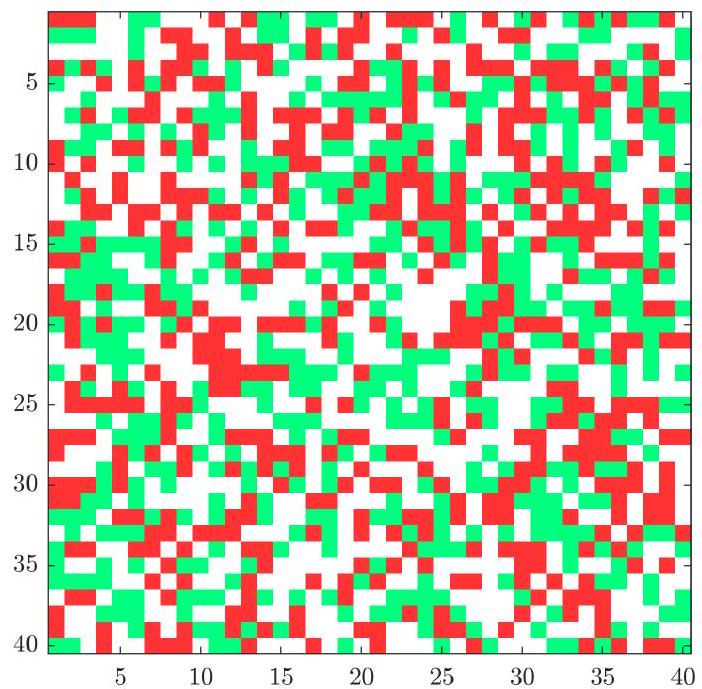
\includegraphics[max width=\textwidth]{2024_03_02_8c82830fbe70d4921a9fg-4(1)}
\end{center}

Figure 1: Initial Configuration.

\begin{center}
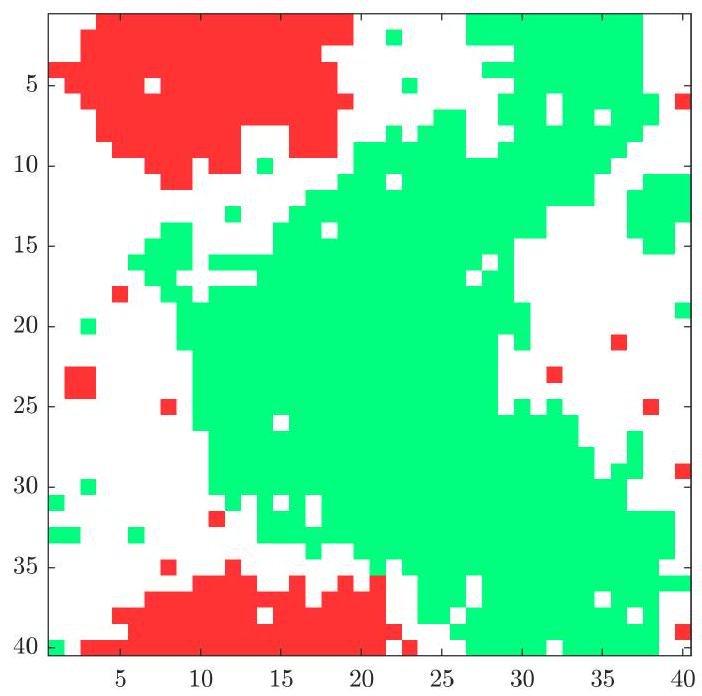
\includegraphics[max width=\textwidth]{2024_03_02_8c82830fbe70d4921a9fg-4}
\end{center}

Figure 2: Final Configuration.

\begin{center}
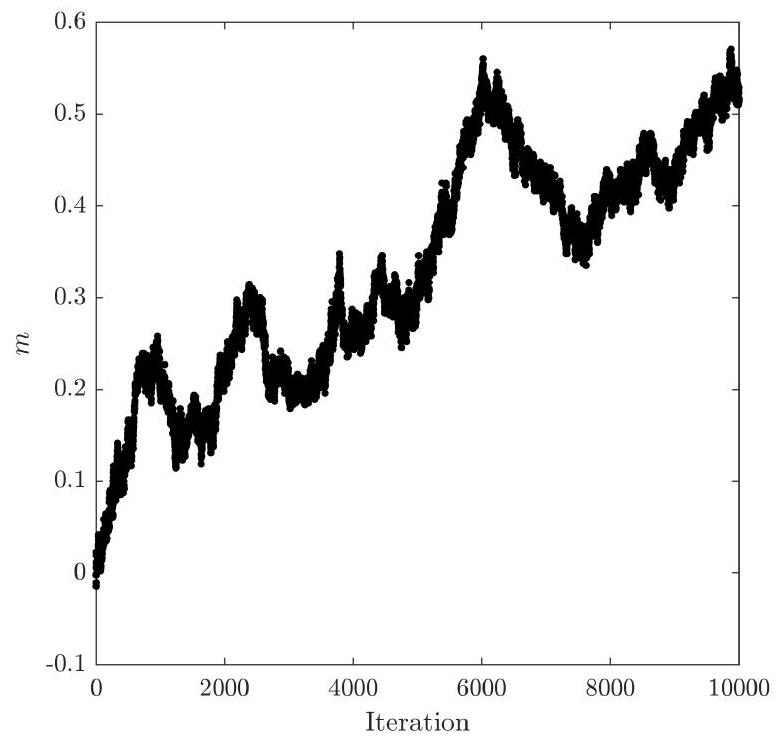
\includegraphics[max width=\textwidth]{2024_03_02_8c82830fbe70d4921a9fg-5(1)}
\end{center}

Figure 3: $m$ vs iter

\begin{center}
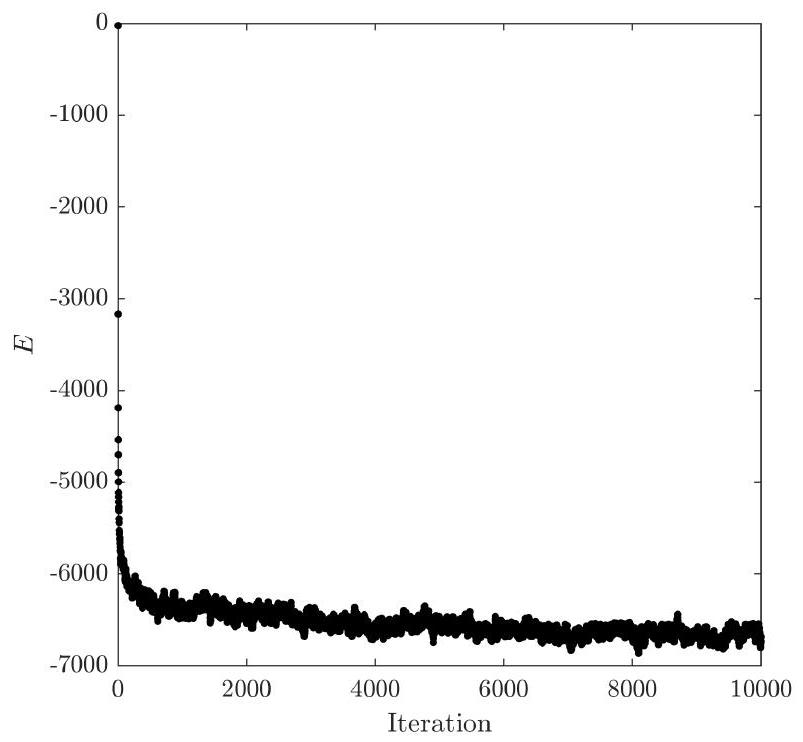
\includegraphics[max width=\textwidth]{2024_03_02_8c82830fbe70d4921a9fg-5}
\end{center}

Figure 4: $E$ vs iter


\end{document}